
\pdfminorversion=4
\documentclass[xcolor=dvipsnames]{beamer}
\usepackage{tabls}
\usepackage{graphicx}
\usepackage{xcolor}
\usepackage{mathtools}
%\usepackage{subcaption}

%tikz stuff
\usepackage{tikz}
\usetikzlibrary{shapes.geometric, arrows}
\tikzstyle{startstop} = [rectangle, rounded corners, minimum width=2cm, text
    width=1.8cm, minimum height=1cm,text centered, text=white,draw=black, fill=Gray!140]
\tikzstyle{io} = [trapezium, trapezium left angle=70, trapezium right angle=110,
minimum width=0.5cm, minimum height=1cm, text centered, draw=black,
fill=blue!20!Gray!90!,text=white]
\tikzstyle{process} = [rectangle, minimum width=2cm, minimum height=1cm, text
centered, text width=2cm, draw=black, text=white,fill=Gray!140!blue!70!white]
\tikzstyle{decision} = [diamond, minimum width=3cm, minimum height=1cm, text
centered, draw=black, fill=Gray!,text=white]
\tikzstyle{arrow} = [thick,line width=0.6mm,->,>=stealth]
\tikzstyle{arrow1} = [dashed,->,>=stealth]

\setbeamertemplate{navigation symbols}{}
\setbeamertemplate{footline}[frame number]
%\setbeamertemplate{headline}{}
\setbeamersize{text margin left=15pt,text margin right=15pt}

\definecolor{mylightlue}{rgb}{1,1,1}
\newcommand*{\boxedcolor}{red}
\makeatletter
\renewcommand{\boxed}[1]{\textcolor{\boxedcolor}{%
  \fbox{\normalcolor\m@th$\displaystyle#1$}}}
\makeatother
\usepackage{hyperref}

\renewcommand{\u}[1]{\underline{#1}}

\newcommand{\iso}[2]{${}^{{#2}}${#1} }
\newcommand{\nubar}[0]{$\overline{\nu}$ }
\newcommand{\keff}[0]{\ensuremath{{k}_{\textsf{eff}}} }
\newcommand{\expect}[1]{E[#1] }
\newcommand{\colg}[1]{{\color{ForestGreen} #1}}
\newcommand{\coly}[1]{{\color{yellow} #1}}
\newcommand{\colb}[1]{{\color{blue} #1}}
\newcommand{\colr}[1]{{\color{red} #1}}
\usepackage{amsfonts}
\newlength{\wideitemsep}
\setlength{\wideitemsep}{8pt}
%\addtolength{\wideitemsep}{5pt}
\let\olditem\item
\renewcommand{\item}{\setlength{\itemsep}{\wideitemsep}\olditem}

\newcommand{\N}{\mathbb{N}}
\newcommand{\Z}{\mathbb{Z}}
\newcommand{\deriv}[2]{\frac{\mathrm{d} #1}{\mathrm{d} #2}}
\newcommand{\pderiv}[2]{\frac{\partial #1}{\partial #2}}
\newcommand{\bx}{\mathbf{X}}
\newcommand{\ba}{\mathbf{A}}
\newcommand{\by}{\mathbf{Y}}
\newcommand{\bj}{\mathbf{J}}
\newcommand{\bs}{\mathbf{s}}
\newcommand{\B}[1]{\ensuremath{\mathbf{#1}}}
\newcommand{\Dt}{\Delta t}
\renewcommand{\d}{\mathsf{d}}
\newcommand{\mom}[1]{\langle #1 \rangle}
\newcommand{\xl}{{x_{i-1/2}}}
\newcommand{\xr}{{x_{i+1/2}}}
\newcommand{\il}{{i-1/2}}
\newcommand{\ir}{{i+1/2}}

\AtBeginSection[]
{
    \begin{frame}<beamer>
        \frametitle{Outline}
        \tableofcontents[currentsection]
    \end{frame}
}

\setbeamerfont{frametitle}{size=\large}
\setbeamerfont{normal font}{size=\small}

\graphicspath{{figures/}}

\usepackage{verbatim}
\usepackage{comment}
\usepackage[]{datetime}
\usepackage{multirow}

\usepackage[]{color}
\usepackage{geometry}

\mode<presentation>
\usepackage{multimedia}

\usepackage{xcolor}


\newcommand{\thedate}{\today}


\setlength{\tabcolsep}{.25cm}

%Aggie-themed
%\pgfdeclareimage[height=0.1in]{TAMUlogo}{tamu_engineering.png}
%\logo{\raisebox{-0pt}{\pgfuseimage{TAMUlogo}}}
\titlegraphic{\centering\begin{tabular}{lr}\includegraphics[height=0.32\textheight]{../graphic/TAMUlogo.png}\end{tabular}}


%%%%%%%%%%%%%%%%%%%%%%%%%%%%%%%%%%%%%%%%%%%%%%%%%%%%%%%%%%%%%%%
% Optional packages, used to show off certain tricks

\newlength \figwidth
\setlength \figwidth {0.5\textwidth}

\setlength{\leftmargin}{0cm}
\setlength{\rightmargin}{0cm}

%%%%%%%%%%%%%%%%%%%%%%%%%%%%%%%%%%%%%%%%%%%%%%%%%%%%%%%%%%%%%%%

\usepackage[english]{babel}
\usetheme{Frankfurt}

%Make it Aggie Maroon
\usecolortheme[RGB={80,0,0}]{structure}  

  % This will typeset only the frames (or slides) that have the given label ("current" in this case).

\title{The Coarse Scattering Method}
    \author{{\Large Pablo A. Vaquer} \vspace{-0.75cm}}
    \date{{22 October 2018}}
\subject{}

\begin{document}

\begin{frame}
    \titlepage 
    \begin{center}
    \end{center}    
\end{frame}


\begin{frame}
\frametitle{The coarse scattering method}

\pause

In the coarse scattering (CS) method, we make the following substitution to the MG transport equation to reduce the size of the scattering matrices
\begin{equation*}
\label{eq:scatter}
\sum_{g'} \Sigma_{s,\ell,g'\to g} \phi_{\ell,g'} \quad \to \quad S_{\ell,e\to g} \sum_{e'} \Sigma_{s,\ell,e'\to e} \phi_{\ell,e'} 
\end{equation*}
where each fine-group $g$ is a subset of a coarse-element $e$ and
\begin{equation*}
\label{Eq.S}
S_{\ell,e\to g}  = \frac{\sum_{g'} \Sigma_{s,\ell,g'\to g} \phi_{\ell,g'}}{ \sum_{e'} \Sigma_{s,\ell,e'\to e} \phi_{\ell,e'}} 
\end{equation*}
\begin{equation*}
\Sigma_{s,\ell,e'\to e} = \sum_{g \in e} \sum_{g' \in e'} \Sigma_{s,\ell,g'\to g} 
\end{equation*}
\begin{equation*}
\phi_{\ell,e} = \sum_{g \in e} \phi_{\ell,g} 
\end{equation*}

\end{frame}

\begin{frame}
\frametitle{The CS method can also be applied to the fission matrix}


For fission, we make the following substitution
\begin{equation*}
\label{eq:fission}
\sum_{g'} \Sigma_{f,g'\to g} \phi_{g'} \quad \to \quad  F_{e\to g} \sum_{e'} \Sigma_{f,e'\to e} \phi_{e'} 
\end{equation*}
where 
\begin{equation*}
\label{Eq.S}
F_{e\to g}  = \frac{\sum_{g'} \Sigma_{f,g'\to g} \phi_{g'}}{ \sum_{e'} \Sigma_{f,e'\to e} \phi_{e'}} 
\end{equation*}
\begin{equation*}
\Sigma_{f,e'\to e} = \sum_{g \in e} \sum_{g' \in e'} \Sigma_{f,g'\to g}
\end{equation*}
\begin{equation*}
\phi_{e} = \sum_{g \in e} \phi_{g} 
\end{equation*}

\end{frame}


\begin{frame}
  \frametitle{Example of fine transfer matrix being decomposed into a coarse transfer matrix and mapping operator}

\begin{figure}[ht]
  \centering
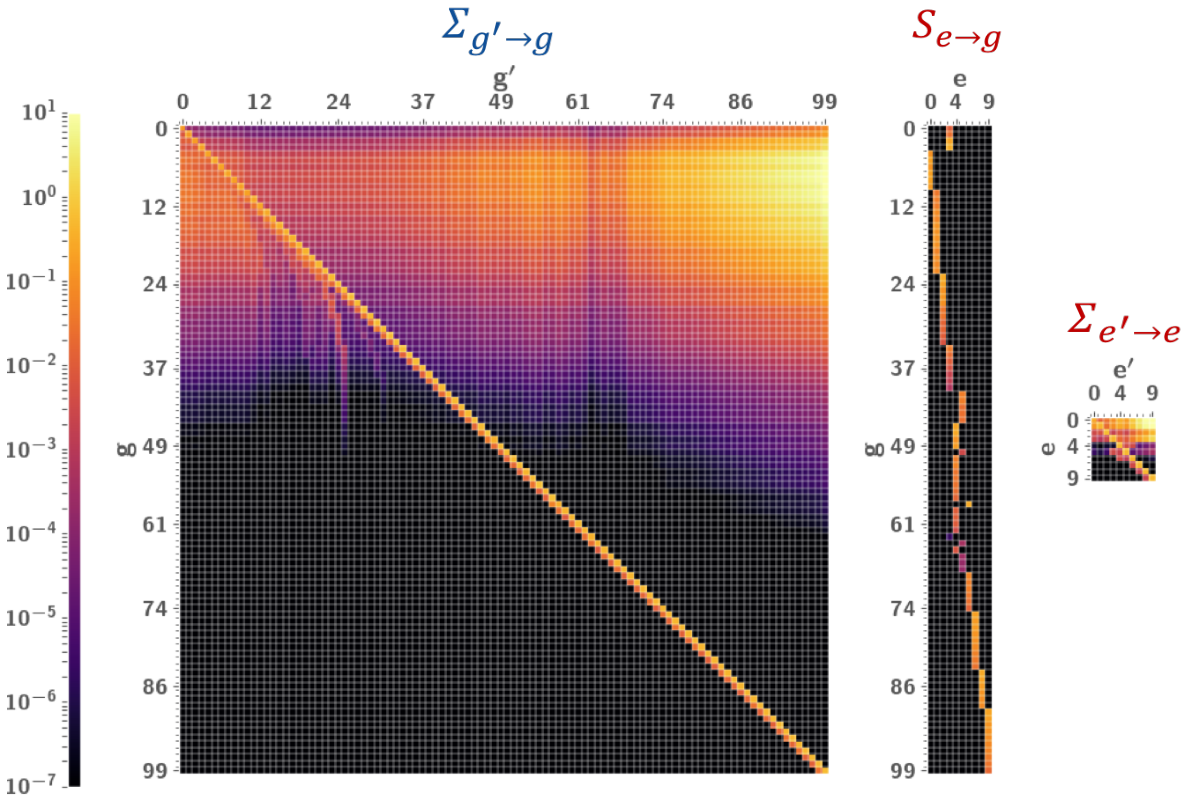
\includegraphics[width=.9\textwidth]{../graphic/matrix_decomposition.png}
\end{figure}
\end{frame}



\begin{frame}
  \frametitle{Recomputing the scattering and fission spectra}

\begin{itemize}
\item Not necessary to recompute both $S_{\ell,e\to g}$ and $F_{e \to g}$ every iteration
\end{itemize}
\begin{multline*}
\label{Eq.feds_transport}
\Bigg[\frac{1}{v_g} \frac{\partial}{\partial t} + \mu \frac{\partial}{\partial x} + \Sigma_{t,g}(\vec{r},t) \Bigg] \psi^{(i+1)}_g(\vec{r},\mu,t)  = q_g(\vec{r},\hat{\Omega},t) + \\ S_{\ell,e\to g}^{(i-s)} \sum_{\ell=0}^L \frac{2 \ell + 1}{2} \sum_{e'} \Sigma_{s,\ell, e' \to e}(\vec{r},t) \phi^{(i)}_{\ell,e'}(\vec{r},t) + \\  \frac{F_{e \to g}^{(i-f)}}{2} \sum_{e'} \Sigma_{f,e' \to e}(\vec{r},t) \phi^{(i)}_{e'}^m(\vec{r},t)
\end{multline*}

\begin{itemize}
\item Asymptotic computational cost of solving the MG transport equation is order $G^2$
\item Asymptotic computational cost of the CS method is order $G$ in iterations when $S_{\ell,e\to g}$ and $F_{e \to g}$ are not recomputed and order $G^2$ only in iterations where $S_{\ell,e\to g}$ and $F_{e \to g}$ are recomputed
\end{itemize}

\end{frame}



\begin{frame}
\frametitle{Particle balance can be maintained}
Particle balance is maintained if following residual $\rho$ is less than machine epsilon in the last iteration,
\begin{multline*}
\label{eq:scatter}
\rho = \Big[ \sum_{g'}  \big( \Sigma_{s,0,g'\to g} + \Sigma_{f,g' \to g} \big)  \phi_{g'} \Big] - \\ \Big[ S_{0,e\to g} \sum_{e'} \Sigma_{s,0,e'\to e} \phi_{e'} + F_{e\to g} \sum_{e'}  \Sigma_{f,e' \to e} \phi_{e'} \Big] 
\end{multline*}
%Our current implementation of the coarse scattering method has reduced the simulation runtime for an infinite-medium eigenvalue calculation by a factor of 6, and reduced the runtime for a 1-D eigenvalue calculation by a factor of 2. The CS method converged to the same MG solution for these simulations. We will explore a few more avenues for achieving even greater reductions in runtime. For example, it may possible to only recompute small portions of $S_{\ell,e\to g}$ and $F_{e \to g}$ from one iteration to the next. Furthermore, it may be possible to design a criterion for when to recompute $S_{\ell,e\to g}$ and $F_{e \to g}$ in order to achieve greater reduction in runtime.

Futhermore, it may be possible to perserve particle balance every iteration if the CS method is only applied to Legendre moments greater than 0
\end{frame}

\begin{frame}
  \frametitle{Preliminary CS Results for a 1D slab of uranium (20$\%$ enriched)}
    \begin{table}[ht]
    \begin{tabular}{c{3.cm}c{1.75cm}c{1.75cm}c{1.75cm}}
    Simulation                                    & MG & CS & CS & CS \\ \\
    Number of Groups                              & 200                 &   200 / 25             &    200 / 5              &    200 / 1       \\ \\
     Recomputations \\ ($S_{e \to g}$ / $F_{e \to g}$)  &                     &    2 / 4               &     2 / 4               &      2 / 4       \\ \\
    $k_{eff}$                                     & $1.15420$           &   $1.15420$            &    $1.15420$            &    $1.15420$      \\ \\
    RHS   Cost                                    & 3.26$\times$10$^8$  &   1.89$\times$10$^8$   &    2.03$\times$10$^8$   &   2.34$\times$10$^8$         \\ \\
    Total Cost                                    & 3.32$\times$10$^8$  &   1.95$\times$10$^8$   &    2.11$\times$10$^8$   &   2.44$\times$10$^8$         \\ \\
    \end{tabular} 
    \end{table}
\end{frame}

\begin{frame}
  \frametitle{Properties of Spherical Harmonics}
\begin{equation*}
\int_{4\pi} d\Omega \, Y_\ell^m(\hat{\Omega}) Y_{\ell'}^{m'}(\hat{\Omega}) = \frac{4\pi}{2\ell + 1} \delta_{\ell \ell'} \delta_{m m'} 
\end{equation*}

\begin{equation*}
\int_{4\pi} d\Omega \, Y_\ell^m(\hat{\Omega}) Y_0^0(\hat{\Omega}) = 4\pi 
\end{equation*}

\begin{equation*}
\int_{4\pi} d\Omega \, Y_\ell^m(\hat{\Omega}) = 4\pi 
\end{equation*}

\end{frame}

\begin{frame}
  \frametitle{Particle balanced is maintain if coarse scattering is only used for higher moments}

\begin{equation*}
\int_{4\pi} d\Omega \, \sum_{\ell = 0}^L \sum_{m = -\ell}^{\ell} \frac{2\ell + 1}{4\pi} Y_\ell^m(\hat{\Omega}) \sum_{g'}^G \Sigma_{s,\ell,g' \to g} \phi_{\ell,g'}^m = \Sigma_{s,0,g' \to g} \phi_{0,g'}
\end{equation*}

\begin{multline*}
\int_{4\pi} d\Omega \, \Big\{ \sum_{g'}^G \Sigma_{s,0,g' \to g} \phi_{0,g'} \: + \\ \sum_{\ell = 1}^L \sum_{m = -\ell}^{\ell} \frac{2\ell + 1}{4\pi} Y_\ell^m(\hat{\Omega}) \sum_{e'}^E \Sigma_{s,\ell,e' \to e} \phi_{\ell,e'}^m \Big\} = \Sigma_{s,0,g' \to g} \phi_{0,g'}
\end{multline*}

\end{frame}





\begin{frame}[noframenumbering]
\frametitle{Thank you}
Questions?
\end{frame}







\end{document}
